\documentclass[crop,tikz]{standalone}
\usetikzlibrary{backgrounds}
\colorlet{blue}{cyan}
\tikzset{
  inverted/.style = {
    every path/.style = {draw=white,text=white},
    background rectangle/.style={fill},
    show background rectangle
  }
}

\tikzset{>=latex}
\newcommand{\place}{\vec{r}}
\newcommand{\F}{\vec{F}}
\colorlet{green}{green}

\begin{document}
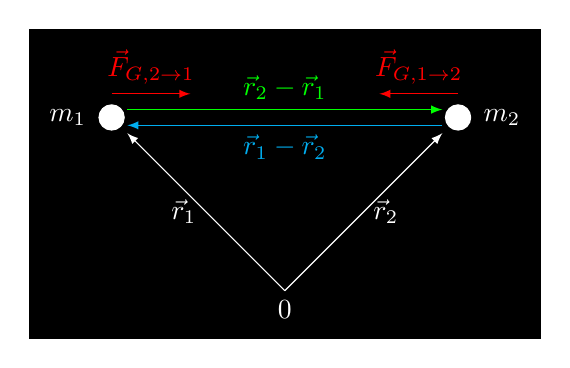
\begin{tikzpicture}[inverted,scale=2]
  \draw[->] (0,0) node[below] {$0$} -- node[left] {$\place_1$} (-1,1);
  \draw[->] (0,0) -- node[right] {$\place_2$} (1,1);
  \draw[fill,white] (-1,1)+(-0.1,0.1) circle (0.08);
  \draw[fill,white] (1,1)+(0.1,0.1) circle (0.08);
  \draw[->,green] (-1,1.15) -- node[above] {$\place_2-\place_1$} (1,1.15);
  \draw[->,blue] (1,1.05) -- node[below] {$\place_1-\place_2$} (-1,1.05);
  \draw (-1.2,1.1) node[left] {$m_1$};
  \draw (1.2,1.1) node[right] {$m_2$};
  \draw[->,red] (-1.1,1.25) -- node[above] {$\F_{G,2\to 1}$} +(0.5,0);
  \draw[->,red] (1.1,1.25) -- node[above] {$\F_{G,1\to 2}$} +(-0.5,0);
\end{tikzpicture}
\end{document}
